This section will give an overview of the main research questions for this project and how I intend to investigate them.
CHECK TENSE IN THIS SECTION

\section{Which aspect types do I use?}
One inherent drawback of computational methods is exactly their one unifying characteristic: their computability. Sadly, the requirement for computability means, in many cases, sacrificing the nuance that comes with more qualitative approaches. In this concrete case this means settling for a single aspect classification system. A consequence of the glut of literature in the field is a glut of classification systems to go with it, each with their own idiosyncrasies and each having their own advantages and drawbacks.

reason is of course the contribution to the linguistic community: computational approaches to language have SPURRED ON LOTS OF PROGRESS (cf Chomsky!!!). 

The classification schema I decided on was Uniform Meaning Representation (UMR) \citep{umr}, for several reasons: On (SHOULD THIS BE CAPITALISED??) the one hand the lattice was designed for ease of annotation and usability and thus does away with a lot of the theoretical baggage of other classification systems (such as the insistence on lexical aspect types). On the other hand the schema is part of a larger framework, and hence a classification system using these labels has a practical application. Furthermore, UMR provides a lattice for annotation (see \ref{fig:umr_aspect_tree}) meaning the level of the annotation classes can be ANGEPASST to the needs of the individual contexts.

\subsection{UMR}
UMR \citep{umr} was introduced in order to expand and further generalise the attempt to design an abstract semantic representation, as was most successfully pioneered by \citet{amr} with Abstract Meaning Representation (AMR). In contrast to AMR, UMR aims to be a typologically-informed abstraction away from English structures, making it more suitable for other similar languages, or, in their own words, making it "a practical and cross-linguistically valid meaning representation designed to meet the needs of a wide range of NLP applications" \citep{umr}.

%WHY IS UMR IMPORTANT???? Get Apaho English comparison from \citet{bonn-etal-2023-mapping}
\subsection*{Aspect in UMR}
\label{aspect_in_umr}
UMR describes the following 5 coarse-grained aspect classes: (descriptions taken from \citet{umr}\footnote{For more detailed descriptions see GUIDELINES LINK!!!!}), also depicted in figure \ref{fig:umr_aspect_tree}:
\begin{itemize}
    \item \textbf{state} - an unspecified type of state
    \item \textbf{habitual} - an event that occurs regularly in the past or
    present, including generic statements
    \item \textbf{activity} - an event that has not necessarily ended and may
    be ongoing at Document Creation Time (DCT)
    \item \textbf{endeavour} - a process that ends without reaching completion
    (i.e., termination)
    \item \textbf{performance} - a process that reaches a completed result
    state
\end{itemize}

\begin{figure}
    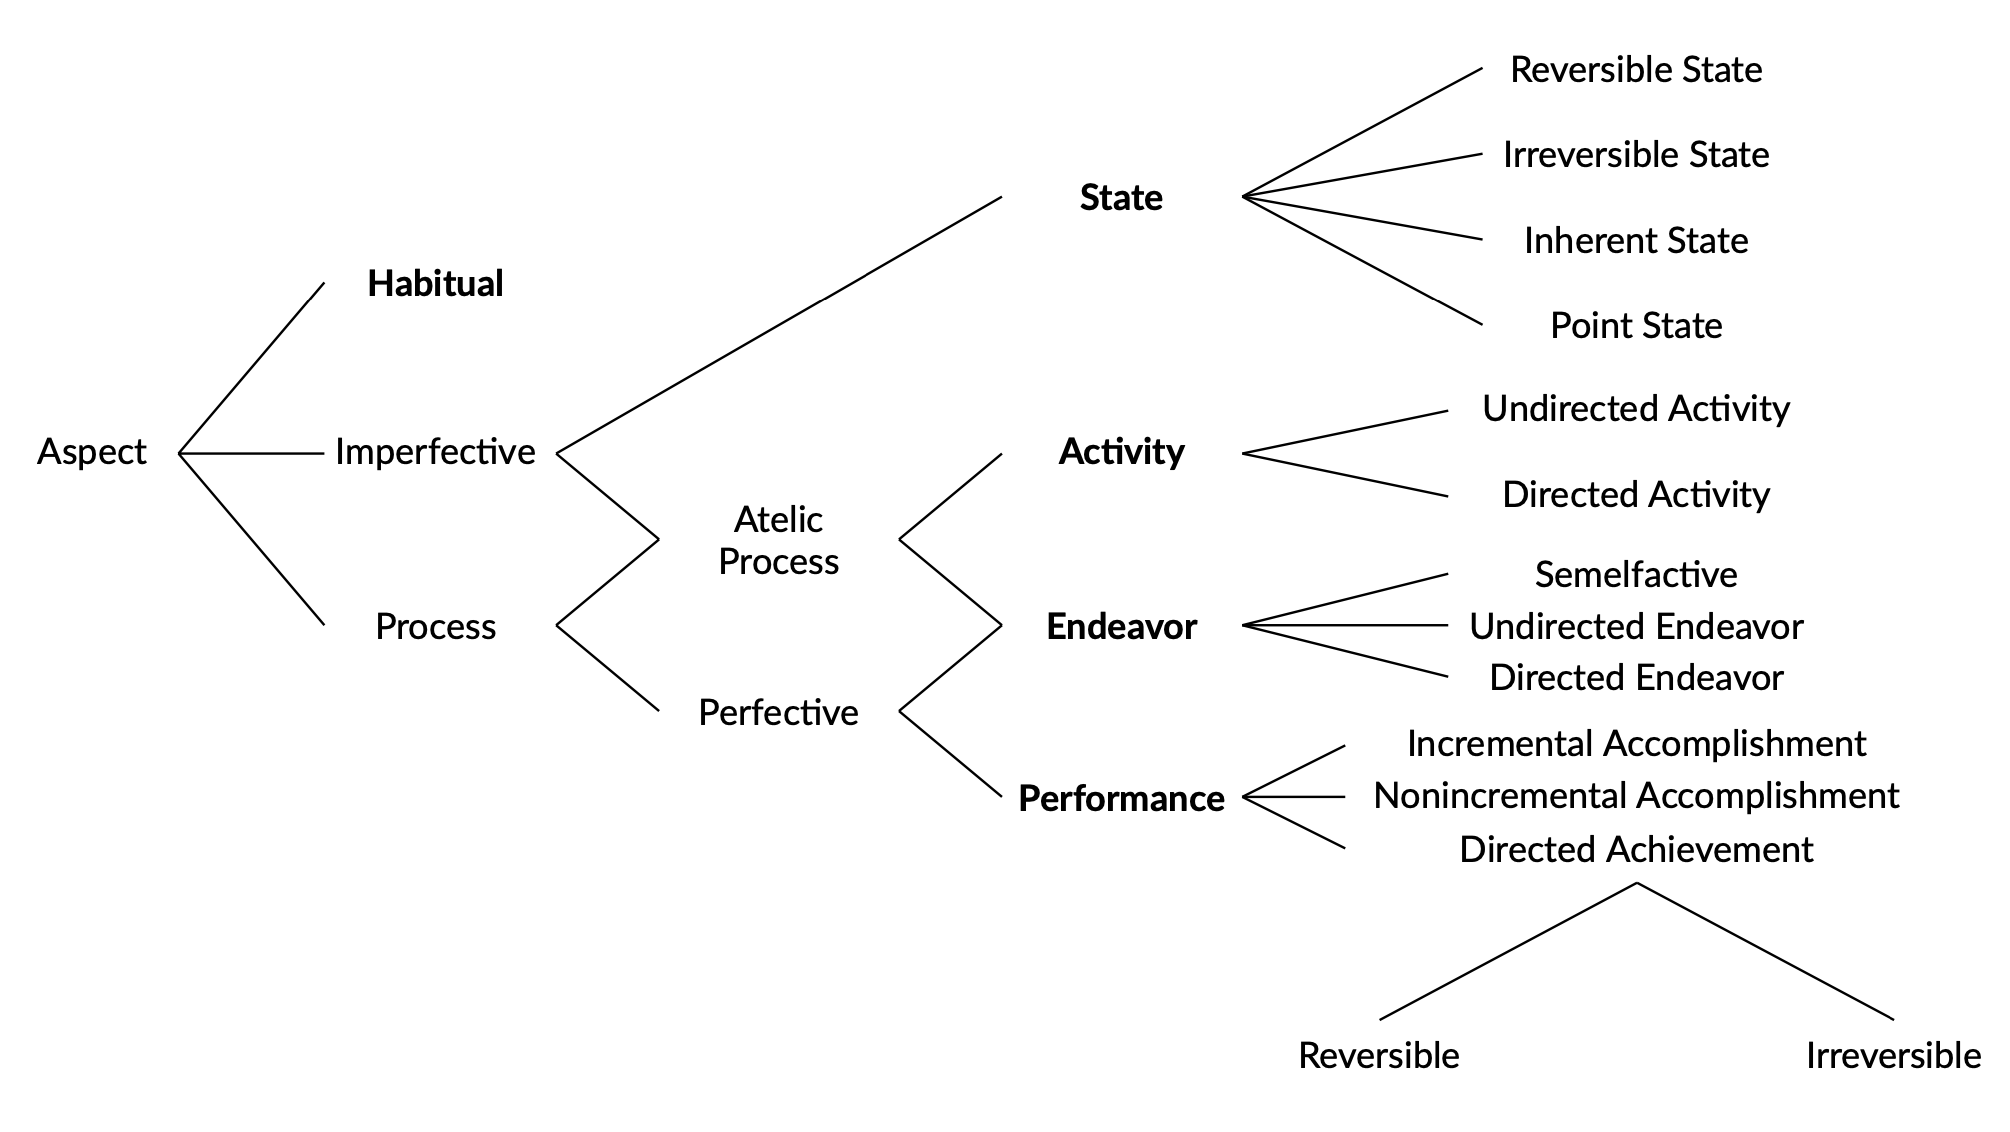
\includegraphics[width=\textwidth]{img/umr_aspct_tree.png}
    \caption{UMR aspect classification lattice \citep{umrslides2022}}
    \label{fig:umr_aspect_tree}
\end{figure}

How these relate to other aspectual classes can be shown in table \ref{table:aspect_classes_comparison}.

Interesting to note is that these classes conflate the distinction made earlier between lexical and grammatical aspect, most clearly in the class "habitual", which is a paradigmatic example of an outer aspect, rather than one inherent in the verb event itself. However, as can be seen in figure \ref{fig:umr_aspect_tree}, while classes which would usually be seen as grammatical aspect are to be found nearer the top of the tree (on the left), the leaves further down the tree are more examples of \emph{Aktionsarten}. That \citet{umr} make no mention of these different types of aspect is not necessarily surprising, given one of the main design goals of UMR being scalability, itself entailing learnability for annotators. As we have seen (HAVE WE?), the theoretical distinction of inner and outer aspect is "very difficult to apply in practice" \citep{Dahl1985TenseAA}, hence a clear separation would often be difficult - and indeed not very fruitful - for annotators. This conflation of two phenomena, however, can also be an advantage, since it shows the relationship between classes of each type (i.e. that \emph{irreversible states} are imperfective and \emph{directed achievements} perfective etc.), subsuming them all into \emph{one} semantic parameter space concerning aspect. A further advantage of UMR is the flexibility of annotation levels that can be seen in figure \ref{fig:umr_aspect_tree}. This allows for annotation both at a fine-grained level (using the classes at the bottom of the tree), but also on a more coarse-grained level if instances are unclear or annotators unsure.

\begin{table}[]
    \begin{adjustbox}{width=\textwidth}
    \begin{tabular}{|l|l|l|l|l|l|l|}
    \hline
    \citet*{vendler57} &  \citet*{moens-steedman-1988-temporal}& \citet*{egg2005flexible} & \multicolumn{3}{l}{\citet*{annotAndAutoClassOfAspectCat}}  \vline & \citet{umr} \\ \hline \hline
\multirow{2}{*}{state}         & state                      & stative predicate     & \multicolumn{3}{l}{stative} \vline & \textbf{state} \\ \cline{2-7}
                               & (habitual state)           & (CHECK THIS)          & \multicolumn{3}{l}{-} \vline & \textbf{habitual} \\ \hline
activity                       & \multirow{2}{*}{process}   & process predicate     & \multirow{5}{*}{dynamic} & \multicolumn{2}{l}{unbounded} \vline & \textbf{activity} \\ \cline{1-1}\cline{3-3}\cline{5-7}
\multirow{2}{*}{accomplishment}&                            & intergressive predicate&      & \multirow{4}{*}{bounded} &  extended/no change & \textbf{endeavour} \\ \cline{2-3}\cline{6-7}
                               & culminated process         & change predicate      &       &  & extended/change & \textbf{performance}\\ \cline{1-3}\cline{6-7}
\multirow{2}{*}{achievement}   & point                      & intergressive predicate&      &  & punctual/no change & \textbf{endeavour} \\ \cline{2-3} \cline{6-7}
                               & culmination                & change predicate      &       &  & punctual/change & \textbf{performance} \\ \hline

    \end{tabular}
    \end{adjustbox}
    \caption{Comparison of aspectual classes. Adapted and extended from \citet*{annotAndAutoClassOfAspectCat}.}
    \label{table:aspect_classes_comparison}
\end{table}

\subsection*{Difficulties with aspect in UMR}
Slightly different to other frameworks (one category can encompass imperfective and perfective?) - is this true

Habitual as aspect

They are not based on classic parameters such as telicity, punctuality etc.

\subsection{How does the Slavic Perfective-Imperfective relate to UMR classes}

Habitual = imperfective
State = imperfective (general imp?)
Activity = imperfective (see motion verbs)
endeavour = 

performance = perfective
\section{Research questions}
\subsection*{RQ1: Can we train a system to identify aspect classes?}
The first question I aimed to look at is whether we can train a system to automatically classify verbs in context as one of several aspect classes. This has been done before (see \ref{sect:previous_asp_class}), however this is the first time that a large language model has been used for this task (CHECK THIS). If this model works well, it will be possible to use it to look at some linguistic questions, such as whether particular prefixes is Slavic languages tend towards certain aspect classes, or carrying out a typological analysis of aspectual ambiguity (RQ3). 
\subsection*{RQ2: Can we automatically identify aspectually ambiguous verbs/sentences and which classes they tend towards?}
Once I have a model which can accurately predict verbal aspect in context, the next question will be the more complex task of predicting aspectual ambiguity, which as far as I am aware, has not been done before. At this stage it is also an interesting question to examine for verb phrases how they are classified without context. This could SHED SOME LIGHT on inherent aspectual readings of verb phrases and thus ANSWER THE QUESTION of whether there are some verb phrases which are perhaps "underspecified" in the model's latent space (see \ref{sect:coerc_or_under}).
\subsection*{RQ3: How does aspectual ambiguity compare across languages? Can we study the typology of aspectualisation?}
Finally, I will attempt to investigate and compare aspectual ambiguity across languages, looking at whether languages with more explicit marking for aspect have less aspect ambiguity than those expressing aspect more implicitly. I plan to answer this both by looking at the ambiguity classification of verbs in context and also of the top \emph{n} verbs in the language without context.
\section{Project outline}
\subsection*{Step 1: Fine-tune LLM for aspect classification}
In order to use language models to investigate aspect, it is necessary to first understand how much current language models know about aspectual phenomena. To this end, I will fine-tune a large language model on a small dataset (since no large datasets are available for the aspect classification scheme I choose, UMR \citep{umr}, or indeed in general for an aspect classification task), testing on a hold-out set. This step of fine-tuning a \emph{large} language model is necessary due to the scarcity of data available, which is not sufficient for fine-tuning a smaller model.
\subsection*{Step 2: Use fine-tuned LLM to annotate larger dataset}
The LLM fine-tuned in step 1 can then be used to annotate a larger dataset. Having a larger dataset allows a great more possibilities for analysis than the dataset used for fine-tuning the larger model. For instance, this larger dataset can be used in a sort of knowledge distillation (KD) process to train a smaller (possibly multilingual) model, which is useful for latent space analysis or comparison across languages. Though it must be noted that there is a danger of error propagation at this step.
\subsection*{Step 3: Compare aspectual systems cross-lingually}
Once we have training data of good enough quality, we can use this to train a multilingual model and use this to compare between languages. Here we can test the model in different contexts and use this to gain insights about the aspect systems of different languages, both in their own right and in comparison with one another, for example, to see if prevalence of aspectual ambiguity changes depending on how overtly a language marks for aspect, or if certain prefixes in a language mark a particular aspect class. Furthermore, 

EQUATION FOR LANGUAGE LEVEL ENTROPY

\subsection*{Step 4: Fine-tune LLM for aspect ambiguity detection}
In order to look at aspect ambiguity specifically, I will also fine-tune an LLM in a similar way to above to identify whether a verb in context has an ambiguous aspectual reading or not. However, since there does not yet exist a dataset annotated for aspectual ambiguity, this part requires human annotation. I propose to solve this by requiring annotators to label sentence-verb pairs with any labels they see plausible. This makes it possible to have both a human class annotation and a derived ambiguity annotation for datapoints labelled with several labels. Neural networks are known for being overly confident in their predictions, and I will investigate whether low certainty of the smaller aspect \emph{classification} model (i.e. similar logit values across classes) correlates with the output of the model specially trained for ambiguity recognition.

\section{Use of approximative LMs as sources of linguistic knowledge?? (Reversing the NLP pipeline)}
Currently the two main approaches used to develop and validate linguistic hypotheses are through corpora and through introspection, the former being championed by empiricists and the latter by the Chomskyan rationalist tradition \citep{corpus_textbook}. It is clear that corpora, including those used to train LLMs, can only contain a fraction of the famously infinite set of possible grammatical sentences in a language, and this has led Chomsky to decry corpus linguistics as seeking to model language \emph{performance} rather than \emph{competence} \citep{corpus_textbook}. Native speaker introspection, on the other hand, while able to judge the grammaticality of any sentence, is clearly highly subjective and biased. Language models, however, are productive and are able to generalize across their corpora to produce, with some sophistication, sentences not seen before in training, thus blurring the line between the traditional Chomskyan distinction between competence and performance. CHANGE THIS WORDING SO ITS NOT WORD FOR WORD AND CITE IT MAYBE??
\section{Where do LLMs fail? (CHANGE - expectation management)} WAS KANN ICH WISSEN? WAS DARF ICH HOFFEN? KANT
It is easy to get 

COPY FROM PAPER?

In light of the current hype surrounding deep learning it is important to highlight the limitations of such techniques and what language models \emph{cannot} do. 

It is well-known that training the LMs discussed in this paper requires a large amount of data and computing resources. While pre-trained models mean that LMs trained on relatively large amounts of data are now available for general use, for less well-resourced languages this is a problem, and their performance suffers drastically. While this does not rule out the use of LMs on such languages (see \citep{kholodna2024llms}), it certainly limits the applicability of some of the uses highlighted in this article, such as for annotation or acceptability analysis.

Furthermore, it must also be noted that LMs take on any biases present in the training data, meaning the language they approximate should be treated with caution. Examining these biases, as has often been done before, can, however, be an area of study in its own right and can produce valuable data for sociolinguistics. However, it must also be noted that it cannot be guaranteed that characteristics of a model's latent space can be transferred to a more general linguistic space, since human linguistic competence and LM competence differ in some aspects. Further research is therefore needed in this area.

Finally, since LMs are trained to minimize error on one variety of a language, they are less well-suited to study linguistic variation, whether geographical or temporal. This makes their use less suitable for languages without an accepted standard variant, such as Swiss German. In these cases, however, an approach using word embeddings such as \citet{hamilton-etal-2016-diachronic} could still be useful. CHANGE WORDING HERE
%\section*{Dataset creation}
%In order to create the dataset for training the model, later to be used for the neural analysis, it is 

%Since UMR aspect is an AMR/UMR node parameter, rather than a clausal one (see for example Smith's situation entity types ADD LINK HERE), it is necessary to first parse any sentence into an AMR graph. However, since no parsers are available for Russian, I had to resort to another option. One possibility would be to develop a system, possibly using tools already available for Russian such as syntax parsers ADD EXAMPLE HERE, however since the focus is on one small part of the AMR/UMR graph - nodes describing an event - this could be an unnecessary distraction. In theory at least, AMR graphs should have a strong correlation with the syntax tree representation of the sentence, and since most events are verbal phrases, this fact can be utilised to simpify the problem. I therefore opted to solve the problem by using a dependency parser (OR SYNTAX PARSER???)